\documentclass[11pt,oneside,abstracton,a4paper]{article}


\usepackage{geometry}
\geometry{left=1.5cm, right=1.5cm, top=2cm, bottom=2cm}


\usepackage{coffee4}
\usepackage{eso-pic}
\usepackage{epsfig,graphicx,subcaption}
\usepackage[
	separate-uncertainty=true,
	per-mode=symbol-or-fraction,
	]{siunitx}
\usepackage{amsmath}
\usepackage{lipsum}


\setcounter{secnumdepth}{2}
\definecolor{DESYorange}{RGB}{242,142,0}
\definecolor{DESYblue}{RGB}{0,166,235}
\definecolor{DESYgrey}{RGB}{119,119,119}
\usepackage[
	colorlinks,
	linkcolor={DESYblue!50!black},
	citecolor={blue!50!black},
	urlcolor={blue!80!black}
	]{hyperref}
\usepackage{pdflscape}
\usepackage{lineno}

\usepackage[
	disable,
	textwidth=3cm
	]{todonotes}
\usepackage{fancyhdr}
\pagestyle{fancy}
\fancyhf{}
\rhead{DESY Summer School 2018}
\lhead{Anja Beck}
\lfoot{Thermal Performance of the Petal Prototype}
\rfoot{\thepage}



%\AddToShipoutPictureBG{
%	\cofeAm{0.2}{1}{0}{-10cm}{-10cm}
%	\cofeDm{0.05}{1}{0}{7cm}{15cm}
%	\cofeCm{1}{1}{0}{1cm}{0cm}
%}

\title{\Large Thermal Performance of the Petal Prototype} 
\author{\normalsize Anja Beck, TU Dortmund, Germany \\[3ex]
DESY Summer Student Programme 2018 \\[3ex]
ATLAS Experiment}
\date{\normalsize \today}

\setlength\parindent{0pt}
\linenumbers
\begin{document}
	\makeatletter
	\begin{titlepage}
		\begin{center}
			\ \\[10ex]
			{\huge \bfseries  \@title }\\[10ex] 
			{\LARGE  \@author}\\[10ex]
			{\large Supervisor: Claire David}\\[10ex]
			{\large \@date}\\[10ex]
			\begin{abstract}
				\noindent
				With the LHC luminosity upgrade, the requirements regarding heat resistance for the detector parts aggravate significantly. To ensure stable measurements and avoid thermal runaway during the measurements, assessing the thermal performance of each of the detector parts is crucial. This report treats the preparations and measurements concerning the thermal behaviour of a petal prototype for the ATLAS inner tracking detector during the Summer Student Programme 2018 at DESY. \\
				\noindent
				This includes determination of the high emissivity coating for the infrared measurements, studies on the theoretical conversion between emitted power and temperature, understanding the camera software, as well as first results of the measurements with the petal.
			\end{abstract}
			\ \\[10ex]
			
\includegraphics[width=0.25\linewidth]{img/DESY_logo_4C.eps}\hspace{20ex}
			
\includegraphics[width=0.25\linewidth]{img/ATLAS-Logo-Square-Blue-RGB.eps} \\[10ex]
%			\renewcommand{\abstractname}{Acknowledgements}
%			\begin{abstract}
%				\noindent
%				
%			\end{abstract}
		\end{center}
	\end{titlepage}
	\makeatother
	\thispagestyle{empty}
	\newpage
	\setcounter{page}{1}

\newpage

\tableofcontents
\newpage
\listoftodos
\newpage
\section{Introduction}
The high-luminosity upgrade for the LHC planned to be ready to run in 2026 imposes new challenges on detectors. For instance, an enhanced luminosity is immediately related to elevated radiation levels which constitute heat development. To avoid a thermal runaway and ensure reliable measurements, the electronics must be held at a constant temperature\todo{How cold should it be?}\ which requires some kind of cooling system for all detector components.

\subsection{Petal}
The summer student project documented in this report was related to the thermal performance tests of the inner tracking detector of the ATLAS experiment. Figure \ref{fig:ATLAS} illustrates its position within the big detector and the planned upgraded design. The parts studied at DESY are the so-called petals that are assembled perpendicularly around the beampipe to track particles with low transversal energy. Figure \ref{fig:petal} displays a picture of the tested petal prototype.
\begin{figure}[h!]
	\centering
	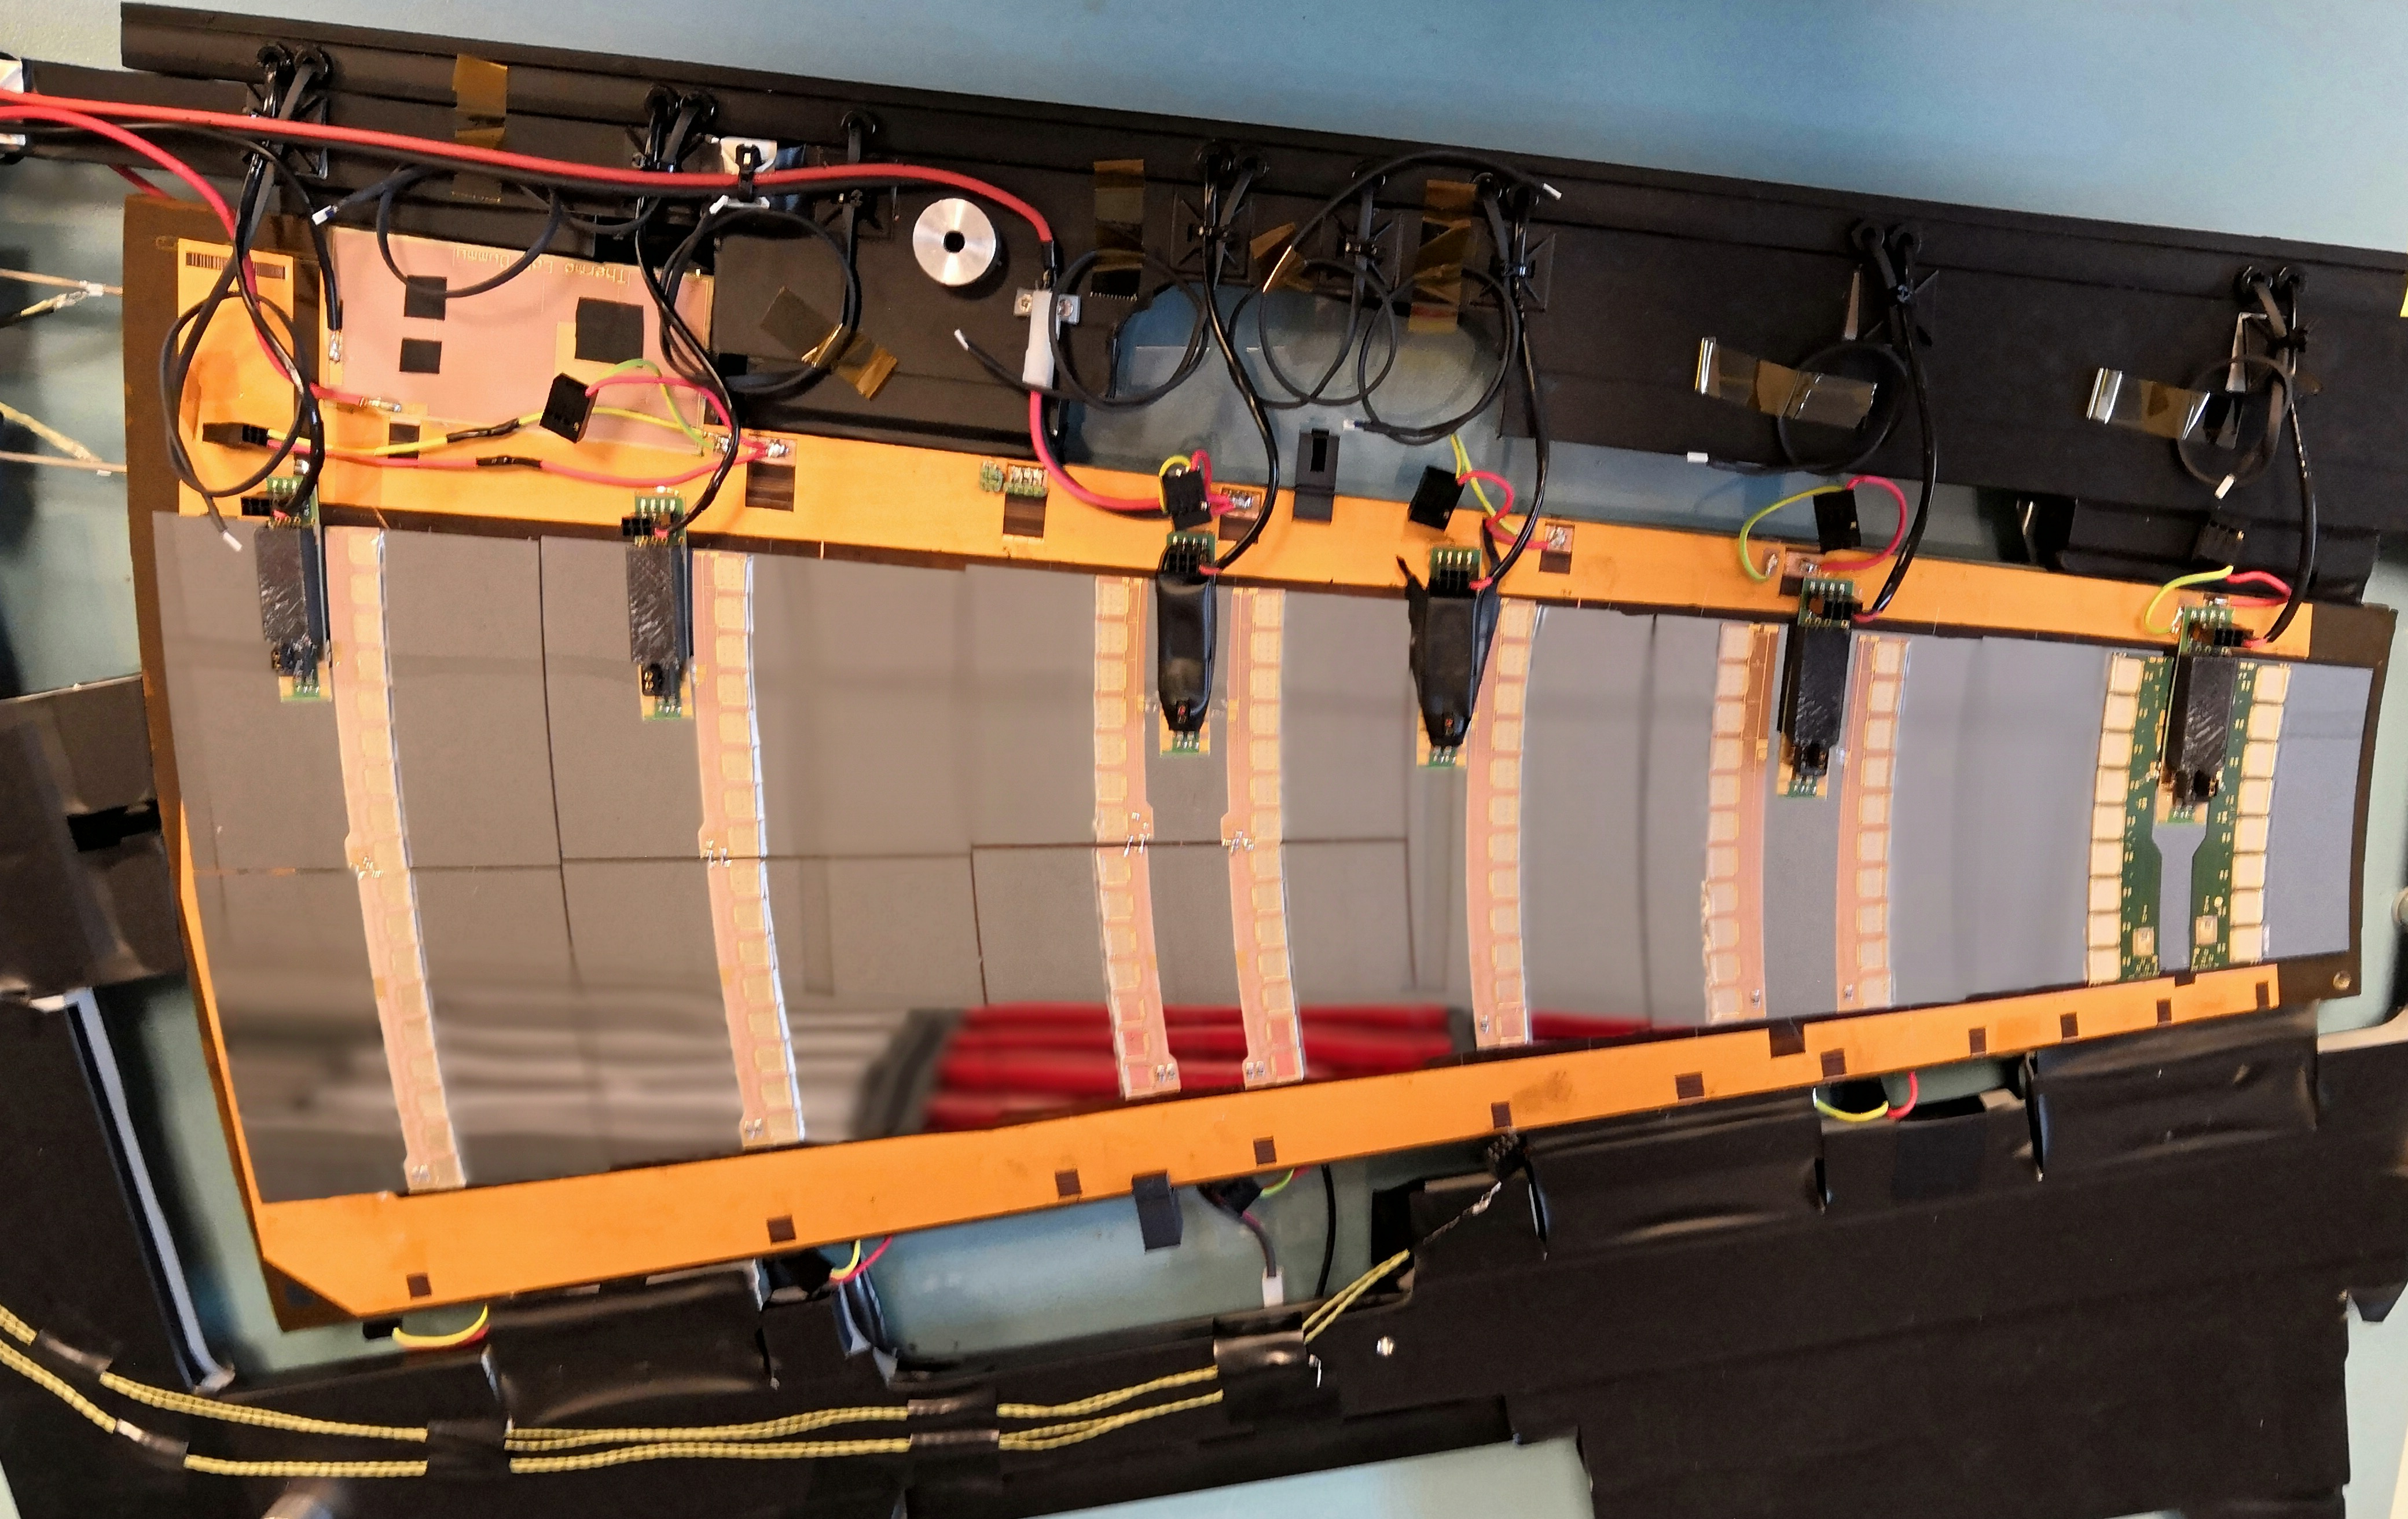
\includegraphics[width=.6\textwidth]{img/petal.jpg}
	\caption{Picture of the tested petal prototype.}
	\label{fig:petal}
\end{figure}
\subsection{Cooling System}
Figure \ref{fig:coolingLoop} shows a prototype of the bare cooling loop. The cooling system is based on the energy needed for a phase change. Liquid $\text{CO}_2$ is pumped into the cooling loop where some of it evaporates if exposed to heat. This evaporation requires energy (enthalpy of evaporation) which is taken from the heat source.
\begin{figure}[h!]
	\centering
	\tikz[baseline=(a.north)]\node[yscale=-1,inner sep=0,outer sep=0](a){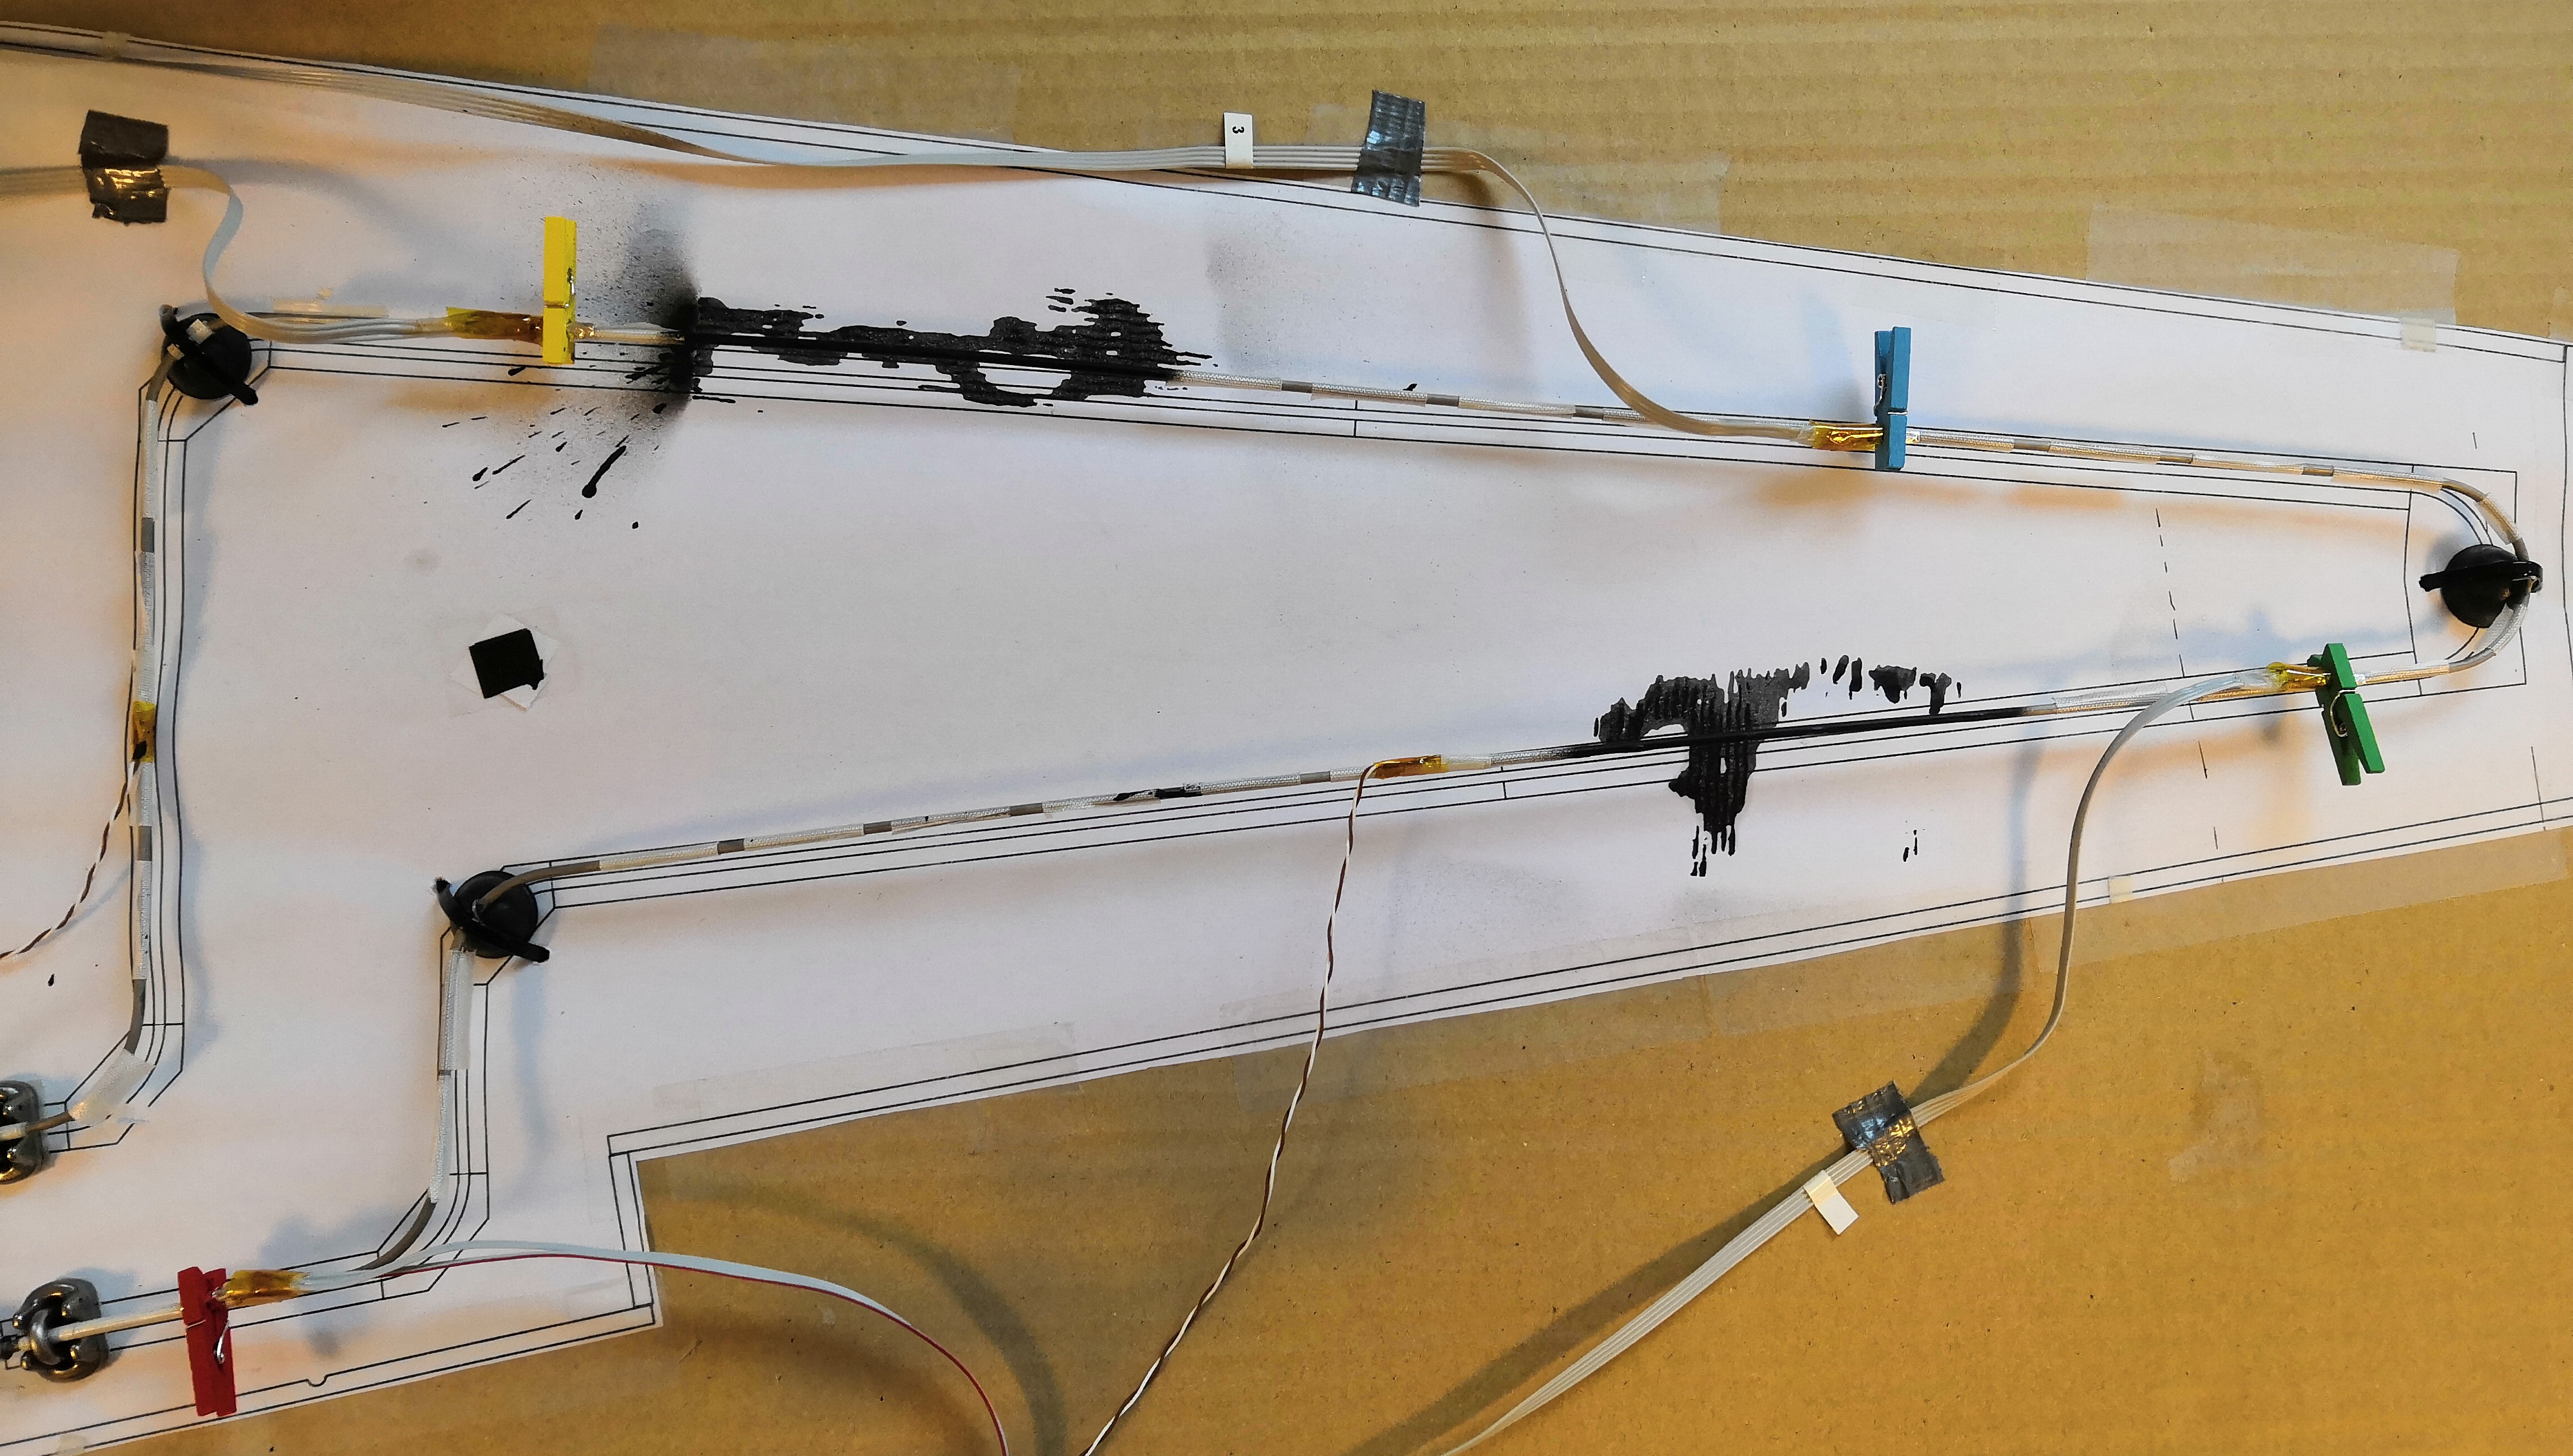
\includegraphics[width=.6\textwidth]{img/coolingLoop.jpg}};
	\caption{Picture of the a bare cooling loop.}
	\label{fig:coolingLoop}
\end{figure}

\begin{landscape}
\begin{figure}[h!]
	\centering
	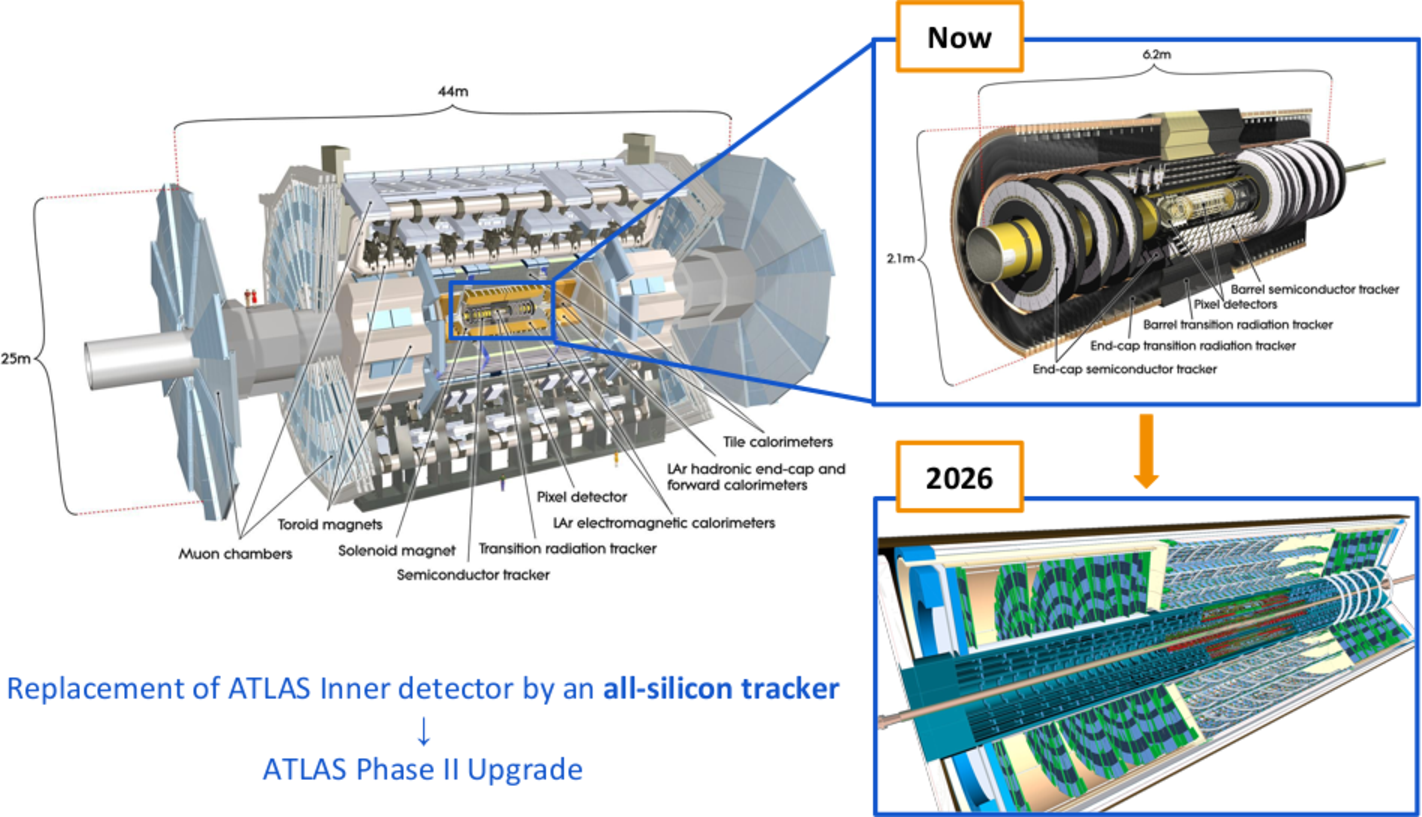
\includegraphics[height=0.9\textwidth]{img/ATLAS.pdf}
	\caption{Schematics of the upgrade of the ATLAS inner tracking detector.}
	\label{fig:ATLAS}
\end{figure}
\end{landscape}

\section{Infrared Theory}
To assess the thermal performance of the petal, we measure the emitted radiation in the infrared (IR) spectrum. To properly evaluate the data measured with the IR camera, we need to understand the behaviour of IR radiation and camera software. This section gives an overview over these topics.
\subsection{Emissivity}
Every body emits IR radiation depending on its temperature. Light in the IR spectrum behaves identical to the more intuitive visible light. This means that surfaces can emit, absorb, and reflect IR radiation. Being purely interested in the \textit{emitted} power, we need to minimize reflection in the IR region. The emissivity $\epsilon$ describes the ability of a surface to reflect IR radiation. \todo{Is it really only IR or is there an emissivity for all ranges?} It is a value between $0$ and $1$, where $0$ corresponds to total reflection, whereas $1$ corresponds to no reflection. So, to achieve good results using IR measurements, we cover the petal with a high emissivity coating. The determination of the exact emissivity value for the chosen paint is described in section \ref{sec:emissivityMeasurement}.

\subsection{Software}

\subsection{Theory}
To fully comprehend and also for being able to check the camera data, a theoretical relation between the emitted power and temperature is crucial. As we are trying to approach an ideal black body using the high emissivity paint, Planck's law for black body radiation,
\begin{align}
	p(\lambda, T) = \frac{2hc^2}{\lambda^5}\frac{1}{\exp\left(hc/(\lambda k_\text{B}T)\right)-1} \ ,
\end{align}
can be a good start. \todo{Describe variables!} The IR camera measures radiation over a range of wavelengths, so we need to integrate this and obtain
\begin{align}
	P(T) = \int_{\lambda_\text{min}}^{\lambda_\text{max}}\frac{C_1}{\lambda^5}\frac{1}{\exp\left(C_2/(\lambda T)\right)-1}\ \text{d}\lambda \ .
\end{align}
Taking account of reflections of the ambiance, we propose the following equation
\begin{align}
	P_\text{tot.}(T) = \underbrace{\epsilon P(T)}_\text{emission} + \underbrace{(1-\epsilon)P(T_\text{amb.})}_\text{reflection of ambiance} \ .
\end{align}\todo{Describe variables!}

\clearpage

\section{Emissivity Measurements\label{sec:emissivityMeasurement}}
This section treats the determination of the emissivity of the paint. To do so, we need the paint to be next to a surface of known emissivity. We use high emissivity tape with $\epsilon_\text{T} = \SI{0.95}{}$. In terms of equation \eqref{eq:powerTemp}, we can then write
\begin{align*}
	P_\text{P} &= \epsilon_\text{P}F(T_\text{P}) + (1-\epsilon_\text{P})F(T_\text{amb}) \text{\quad for the paint,} \\
	P_\text{T} &= \epsilon_\text{T}F(T_\text{T}) + (1-\epsilon_\text{T})F(T_\text{amb}) \text{\quad for the tape.}
\end{align*}
Assuming that both areas have the same real temperature because of their proximity and therefore emit the same amount of IR radiation, we set $P_\text{P}=P_\text{T}$. After rearranging, we obtain an equation for the emissivity of the paint
\begin{align}\label{eq:emissivity}
	\epsilon_\text{P} = \epsilon_\text{T}\frac{F(T_\text{T})-F(T_\text{amb})}{F(T_\text{P})-F(T_\text{amb})} \ .
\end{align}
%The surface temperatures $T_\text{P}, T_\text{T}$ are measure


In the following, we first describe the used set-up for measuring the emissivity of the paint and afterwards analyse the obtained data.
\subsection{Set-Up\label{sec:setup}}
As the petal will later be used at temperatures below \SI{0}{\degreeCelsius}, the thermal performance tests need to be adapted to low temperatures too. Therefore, we measure the emissivity of the paint on the cold side of a Peltier element. Actually, we use two Peltier elements next to each other covered by aluminium plates on the both sides. For simplicity, we shall refer to this combination of Peltier elements as 'the Peltier'. Figure \ref{fig:peltier} shows its cold side with the tape and paint. Additionally, we measure the surface temperature with pt100s. These values are a reference to the IR measurements and to control the Peltier. We calculate the emissivity with the IR data to guarantee comparability with the petal measurements which due to practical reasons cannot be done by pt100s all over the petal. \\


\begin{figure}[h!]
	\centering
	\includegraphics[width=0.8\textwidth]{img/PeltierCloseUp.png}
	\caption{Peltier element used for measuring the emissivity of the paint. We see the cold side with a taped and a painted area. There are also for thermocouples (type: pt100) which are named according to their position (e.g. TL means tape left). Additionally there is an IR camera measurement area next to each of the thermocouples.}
	\label{fig:peltier}
\end{figure}


\todo[noline]{Is the chiller also to reach lower temperatures?}
To ensure a low humidity to avoid ice formation, the Peltier sits in a cardboard box with dry air flushing that only leaves a hole for the camera lens. Furthermore to secure an optimal cooling of the Peltier, we cool its warm side using a chiller. \\


To gather the needed data, we run a current through the Peltier and wait some minutes until the pt100s and the voltage stabilise. Then we note the pt100 values as well as the temperature and radiance power for the four measurement areas as computed by the software. Additionally, we measure the ambient temperature and relative humidity in the box. We stop the measurement when the Peltier stops cooling efficiently (no stable minimum) or when ice forms on the Peltier. \\


We ran this routine three times trying to lower the humidity. Using humidity pearls worked well. Covering the inside walls of the cardboard box with acrylic glas did not lead to any improvement.
\subsection{Results}
Figure \ref{fig:emissivity} shows the results for the emissivity of the paint for all three runs. The values are all quite stable within the runs but vary a lot among them. We have no explanation for this yet.
\begin{figure}[h!]
	\centering
	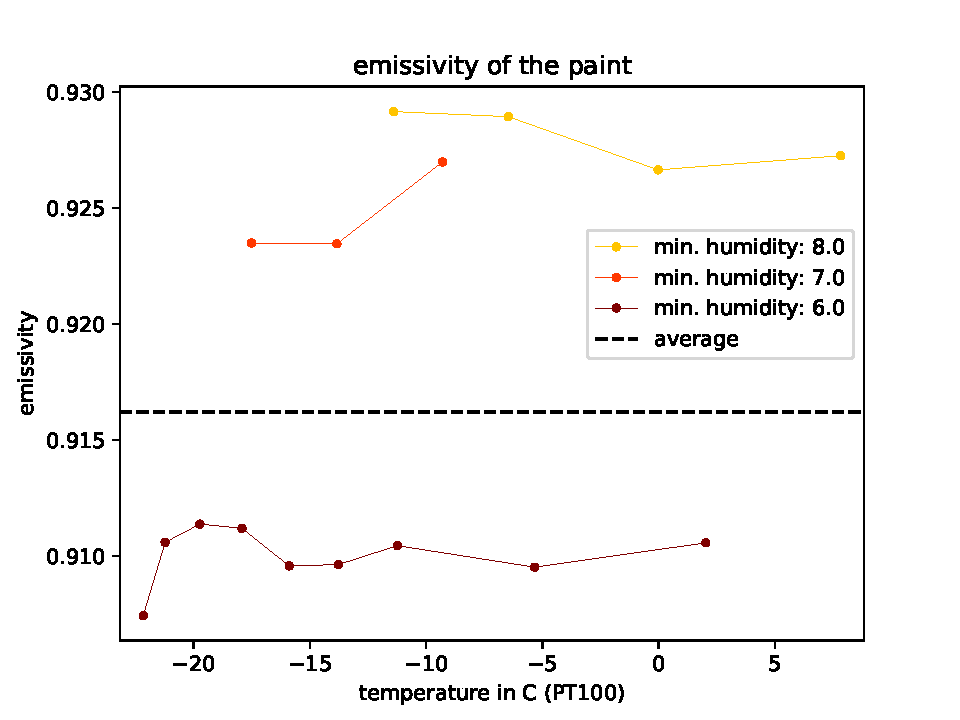
\includegraphics[width=0.7\textwidth]{img/emissivity.pdf}
	\caption{Emissivity values for the three different measurement runs with their absolute average.}
	\label{fig:emissivity}
\end{figure}


Figure \ref{fig:tempTemp} displays the difference in temperature between the pt100s and the corresponding IR measurement point taken at the respective emissivity value. For the tape values, this is mostly within the acceptable range of \SI{1}{\degreeCelsius} deviation. For the paint values the deviation reaches more than \SI{4}{\degreeCelsius}. Given the good result for the tape, we suspect our emissivity value of 0.920 to be wrong.
\begin{figure}[h!]
	\centering	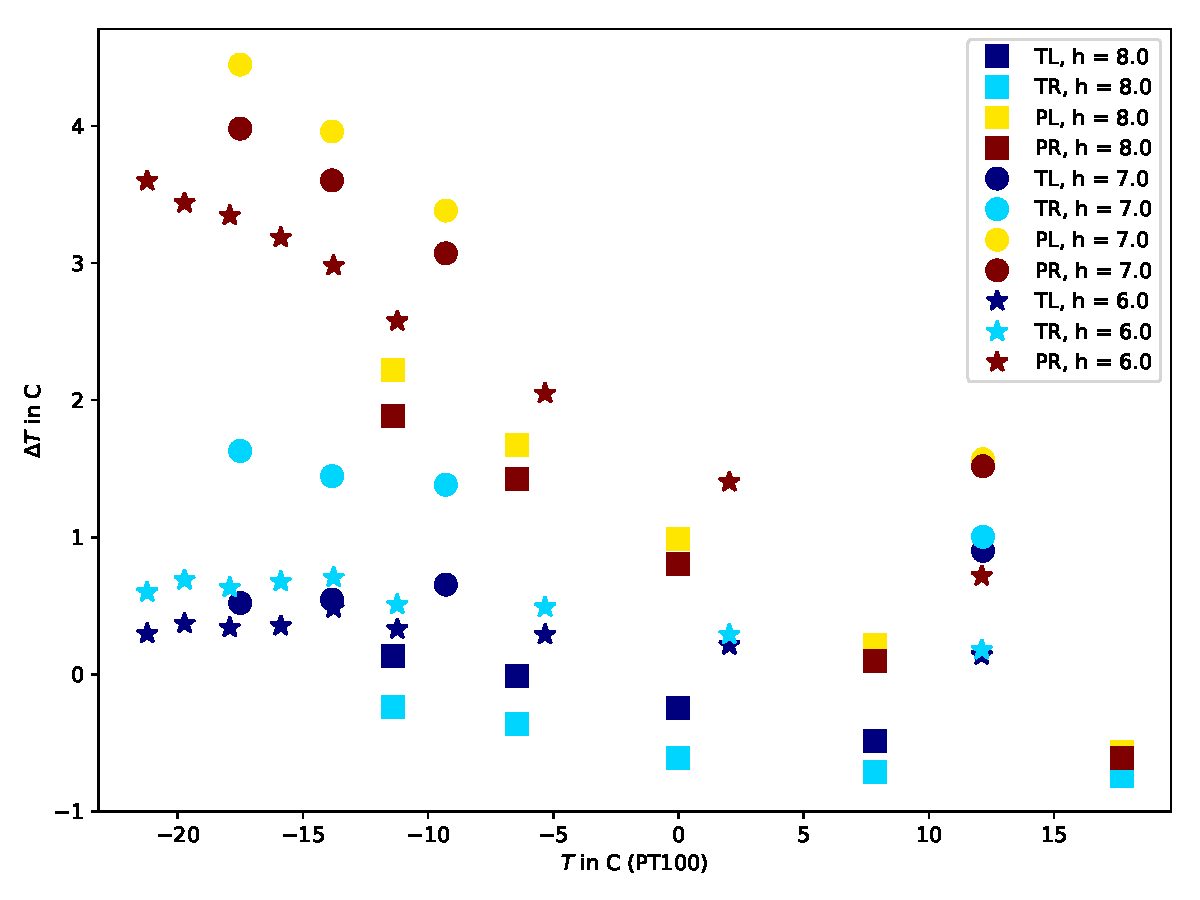
\includegraphics[width=0.8\textwidth]{img/temp_diff_oneplot.pdf}
	\caption{Temperature difference $\Delta T$ for all available data points in the three different measurement runs. For the tape the emissivity is set to \SI{0.95}{}, for the paint it is  \SI{0.92}{}.}
	\label{fig:tempTemp}
\end{figure}
\section{Understanding the Camera Software}
\todo{Check how this goes!}
When reaching the camera sensor, the IR photons induce a current. The software interprets this signal and displays the corresponding temperature. According to the user's manual, these computations are based on equation \eqref{eq:powerTemp} (see section \ref{sec:theory}). As described in section \ref{sec:theory}, we are not yet able to reproduce the camera data with it. \\


To gain confidence in the software nevertheless and intuition for crucial variables in infrared measurements, we conducted studies using the camera software. Figure \ref{fig:softwareClean} shows the result. To obtain it, we took one of the thermograms taken during the emissivity measurements described in section \ref{sec:emissivityMeasurement} and chose one measurement point (paint right)\todo{What temperature was the thermogram taken at?}. We then manually set different ambient temperatures and varied for each of them the emissivity, keeping all other variables constant. In brief, the plot shows the dependence of the object temperature on ambient temperature and emissivity.
\begin{figure}[h!]
	\centering
	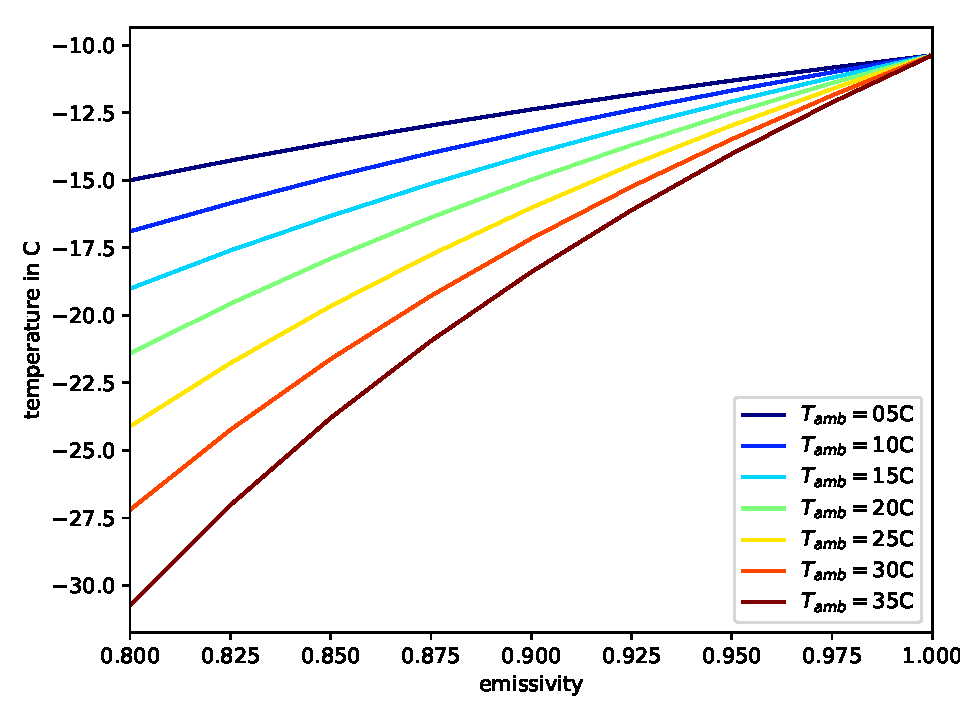
\includegraphics[width=.8\textwidth]{img/softwareClean.pdf}
	\caption{Object temperature on the paint for different emissivities and ambient temperatures computed by the software.}
	\label{fig:softwareClean}
\end{figure} \\

Figure \ref{fig:softwareTape} shows the same plot using the same thermogram but using tape right as measurement point. As pointed out by the red dotted line, the emissivity for this measurement with real $T_\text{amb}=\SI{21.9}{\degreeCelsius}$ and real surface temperature $T_\text{pt100} = \SI{-11.54}{\degreeCelsius}$ should roughly be \SI{0.96}{}. This is close but not identical to the manufacturer value of \SI{0.95}{}.\todo{Comment this result.}
\begin{figure}[h!]
	\centering
	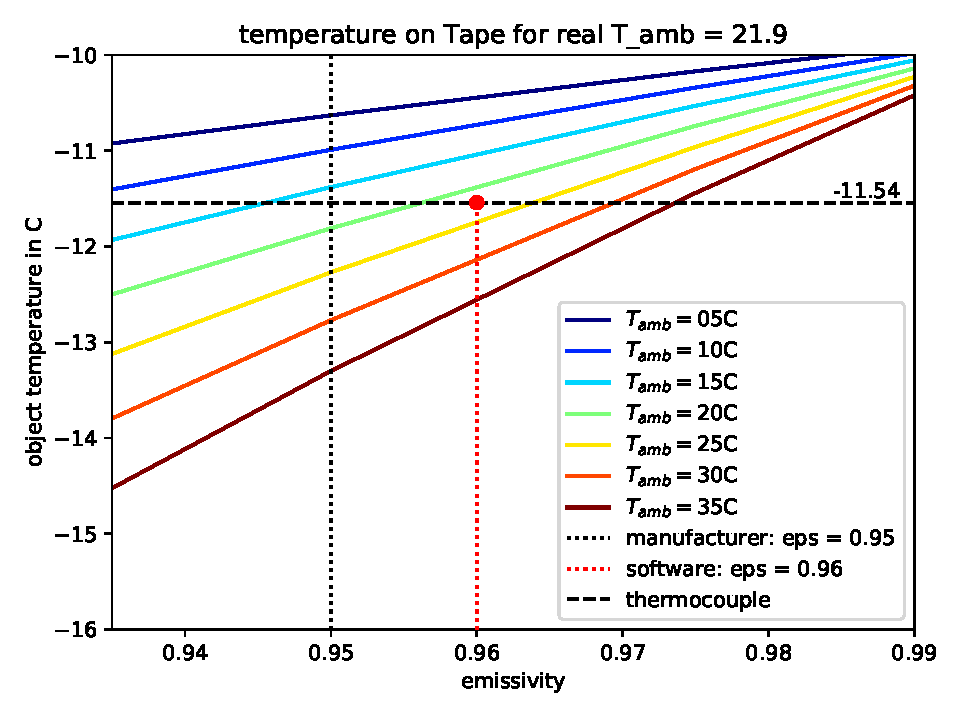
\includegraphics[width=.8\textwidth]{img/softwareTape.pdf}
	\caption{Object temperature on the tape for different emissivities and ambient temperatures computed by the software.}
	\label{fig:softwareTape}
\end{figure} \\


If we go back to the paint, we can use this kind of plot to evaluate the impact of the uncertainty in the emissivity value (see section \ref{sec:emissivityMeasurement}) on the temperature measurement. Figure \ref{fig:softwarePaint-10} shows again the dependency of temperature on the paint on ambient temperature and emissivity. Assuming $T_\text{amb}=\SI{20}{\degreeCelsius}$, the emissivity range and the following temperature range is being highlighted by the orange dotted lines. More precisely, the emissivity range of $0.905\leq\epsilon\leq0.930$ determined in section \ref{sec:emissivityMeasurement} leads to a temperature uncertainty of just above \SI{1}{\degreeCelsius} at a real surface temperature of roughly $T_\text{pt100} = \SI{-10}{\degreeCelsius}$ (see \ref{fig:softwarePaint-10}). For colder temperatures around $T_\text{pt100} = \SI{-20}{\degreeCelsius}$, the following temperature uncertainty rises to \SI{2}{\degreeCelsius}.\todo{Comment on this result.}
\begin{figure}[h!]
	\centering
	\begin{subfigure}{0.5\textwidth}
		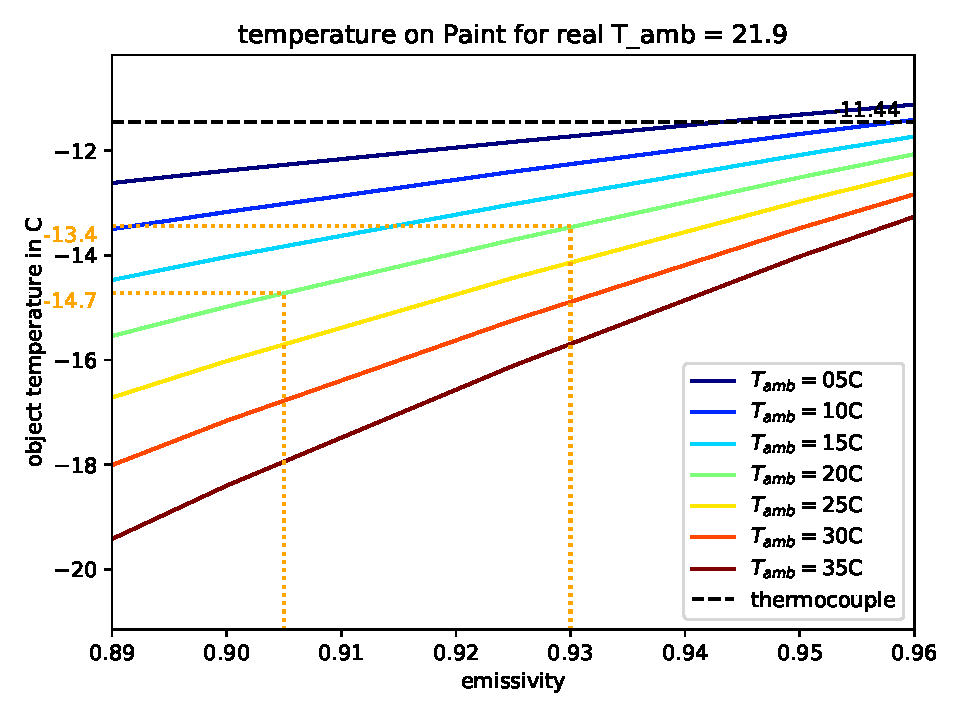
\includegraphics[width=.8\textwidth]{img/softwarePaint-10.pdf}
		\caption{$T_\text{pt100} = \SI{-11.44}{\degreeCelsius}$.}
		\label{fig:softwarePaint-10}
	\end{subfigure}%
	\begin{subfigure}{0.5\textwidth}
		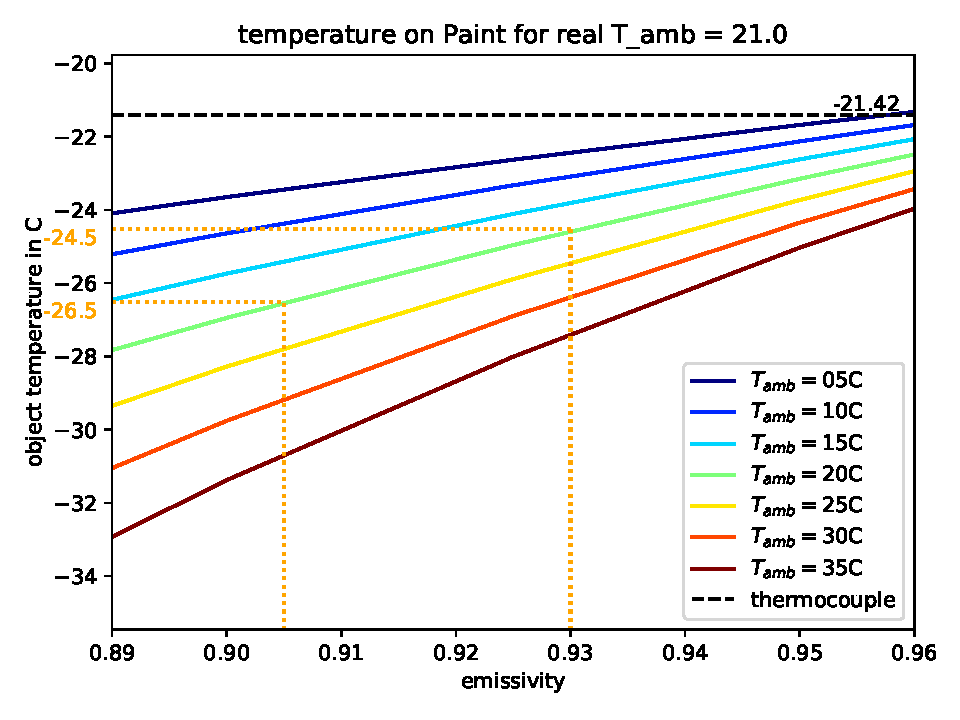
\includegraphics[width=.8\textwidth]{img/softwarePaint-20.pdf}
		\caption{$T_\text{pt100} = \SI{-21.42}{\degreeCelsius}$.}
		\label{fig:softwarePaint-20}
	\end{subfigure}
	\caption{Object temperature on the paint for different emissivities and ambient temperatures computed by the software, including a display of the effect of an uncertainty in the emissivity on the temperature for an ambient temperature of \SI{20}{\degreeCelsius}.}
	\label{fig:softwarePaint}
\end{figure} \\
\clearpage
\section{Tests on the Petal}
This section treats the preparation of the petal in the first two subsections and eventually the first results of the thermal performance tests done in late august 2018 in the third subsection.
\subsection{Last Pre-Study on Gluing pt100s and Paint Emissivity on Si}
As outlined in section \ref{sec:emissivity}, the petal needs to be covered with a high emissivity coating. The chosen paint was examined in section \ref{sec:emissivityMeasurement}.
Before the tests could start, we decided to do a last pre-study to check if the paint when sprayed onto Si has the same emissivity as on Aluminium and to check if gluing the pt100s onto Si is as reliable as clamping. The set-up for this test is similar to the one described in \ref{sec:setup}: the same Peltier element sitting in the same cardboard box. The only modifications are on the surface of the Peltier as shown in figure \ref{fig:peltierGlue}.
\begin{figure}[h!]
	\centering
	\includegraphics[width=0.6\textwidth]{img/peltierGlued.png}
	\caption{Cold side of the Peltier to test the emissivity of the paint on Si and the reliability of glued pt100s. The Si plate has two parts: one unpainted side with three glued and one clamped pt100, and one painted side with six IR measurement areas. The green and blue squares represent the IR measurement areas on the tape and paint.}
	\label{fig:peltierGlue}
\end{figure}
\subsubsection{Reliability of Glued pt100s}
Figure \ref{fig:glueTemp} compares the temperature measurement of the three glued pt100s and the one clamped pt100s on the Si plate. One of the glued pt100s shows a large deviation whereas the two remaining glued pt100s are rather close to the clamped one. We consider gluing to be a trustworthy measurement overall.
\begin{figure}[h!]
	\centering
	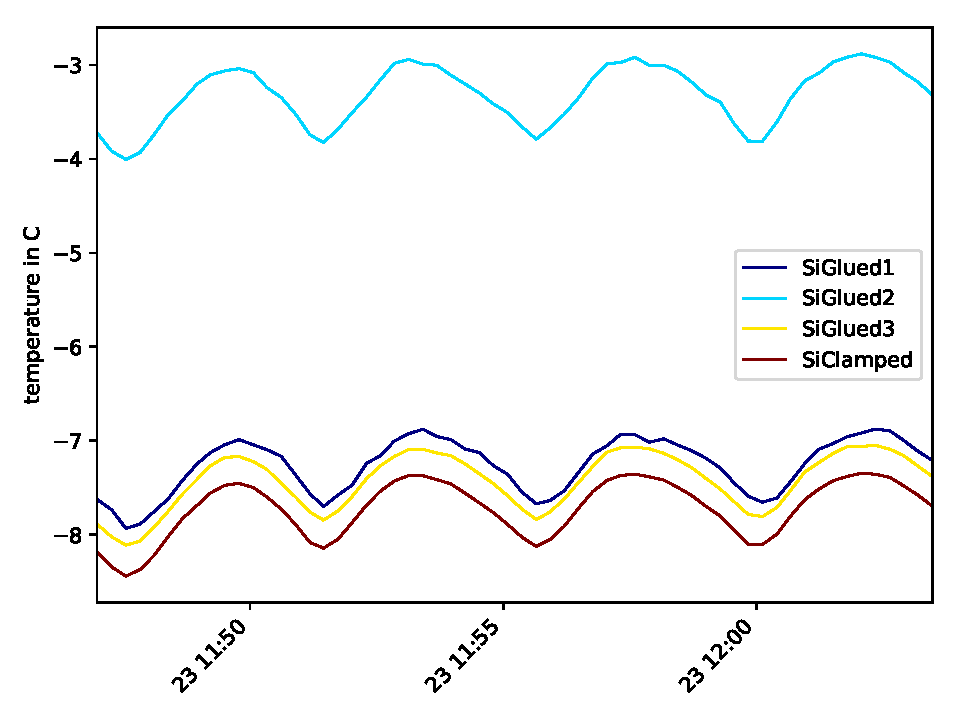
\includegraphics[width=0.7\textwidth]{img/gluing.pdf}
	\caption{Temperatures as measured by the three glued and the one clamped pt100s on the Si.}
	\label{fig:glueTemp}
\end{figure}



\subsubsection{Emissivity of the Paint on Si}
To obtain an emissivity value for the paint on Si, we use again equation \ref{eq:emissivity}, comparing the Si measurement areas with the rightmost tape area. Additionally, we compute again emissivities for the paint on aluminium, comparing each paint area with the closest tape area. Figure \ref{fig:emissivitySi} shows the resulting emissivities. Notably, the values are relatively stable over a broad temperature range and the values for the paint on aluminium are in the range determined in section \ref{sec:emissivityMeasurement}. We expect to have the same emissivity independent of the underlying material. Unfortunately, the emissivities of the paint on Si are higher than this range. We suspect reflections of the clamps, the glue, and the shiny uncoated part of the Si plate to possibly have caused this result. The grouping of the values for the three left and right Si measurement areas supports this argument.
\begin{figure}[h!]
	\centering
	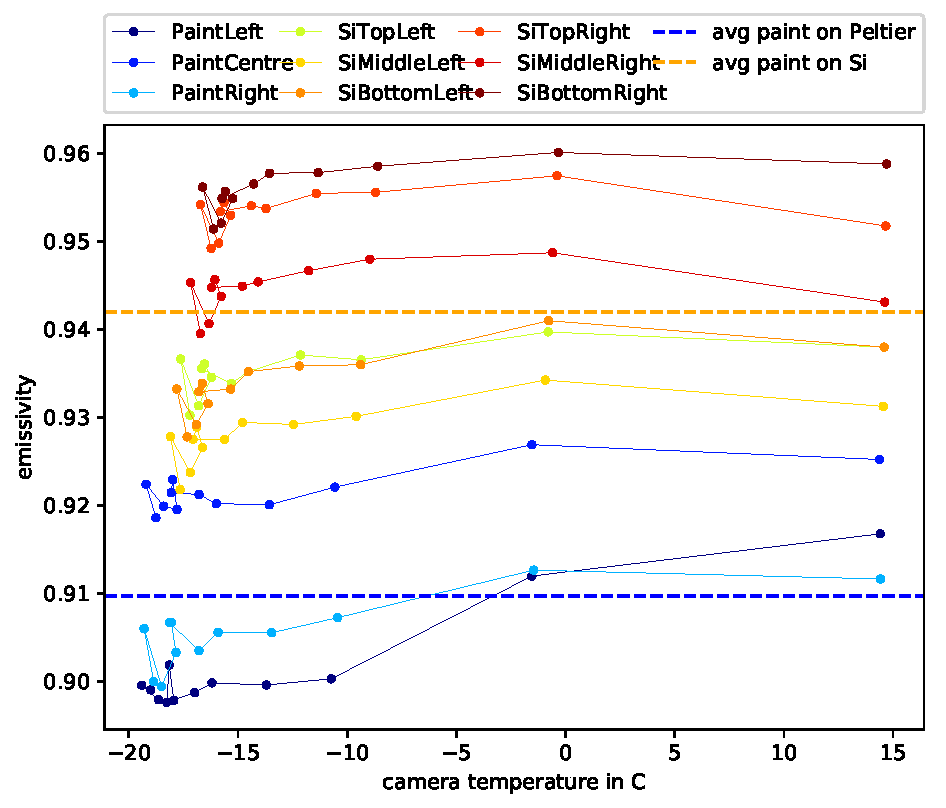
\includegraphics[width=0.7\textwidth]{img/emissivitySi.pdf}
	\caption{Emissivity values for the paint on the Peltier (aluminium) and paint on the Si plate.}
	\label{fig:emissivitySi}
\end{figure}

\subsection{Spraying the Petal}
Intuitively, one would spray the paint onto the petal by laying it on a horizontal surface and spraying from above. This would lead the paint to distribute evenly due to gravitational forces and give a sleek layer of paint. However, number one priority in the spraying process is preserving the wirebonds and the electronics in general. Having a big amount of liquid paint on the petal seems to be too risky which is why we choose to apply the paint from a distance while the petal is in a horizontal position. In figure \ref{fig:petalPreAndPost}, we see the petal before and after the spraying procedure. Figure \ref{fig:petalCloseUp} illustrates the downside of the technique describe above: The paint layer is quite rough and sandy. This does not interfere with the IR measurements given that we cannot observe any Narcissus effect\footnote{Seeing the reflection of the heat emitted by the IR camera in the thermogram when looking at the surface perpendicularly is called Narcissus effect.}.
\begin{figure}[h!]
	\centering
	\begin{subfigure}{\textwidth}
		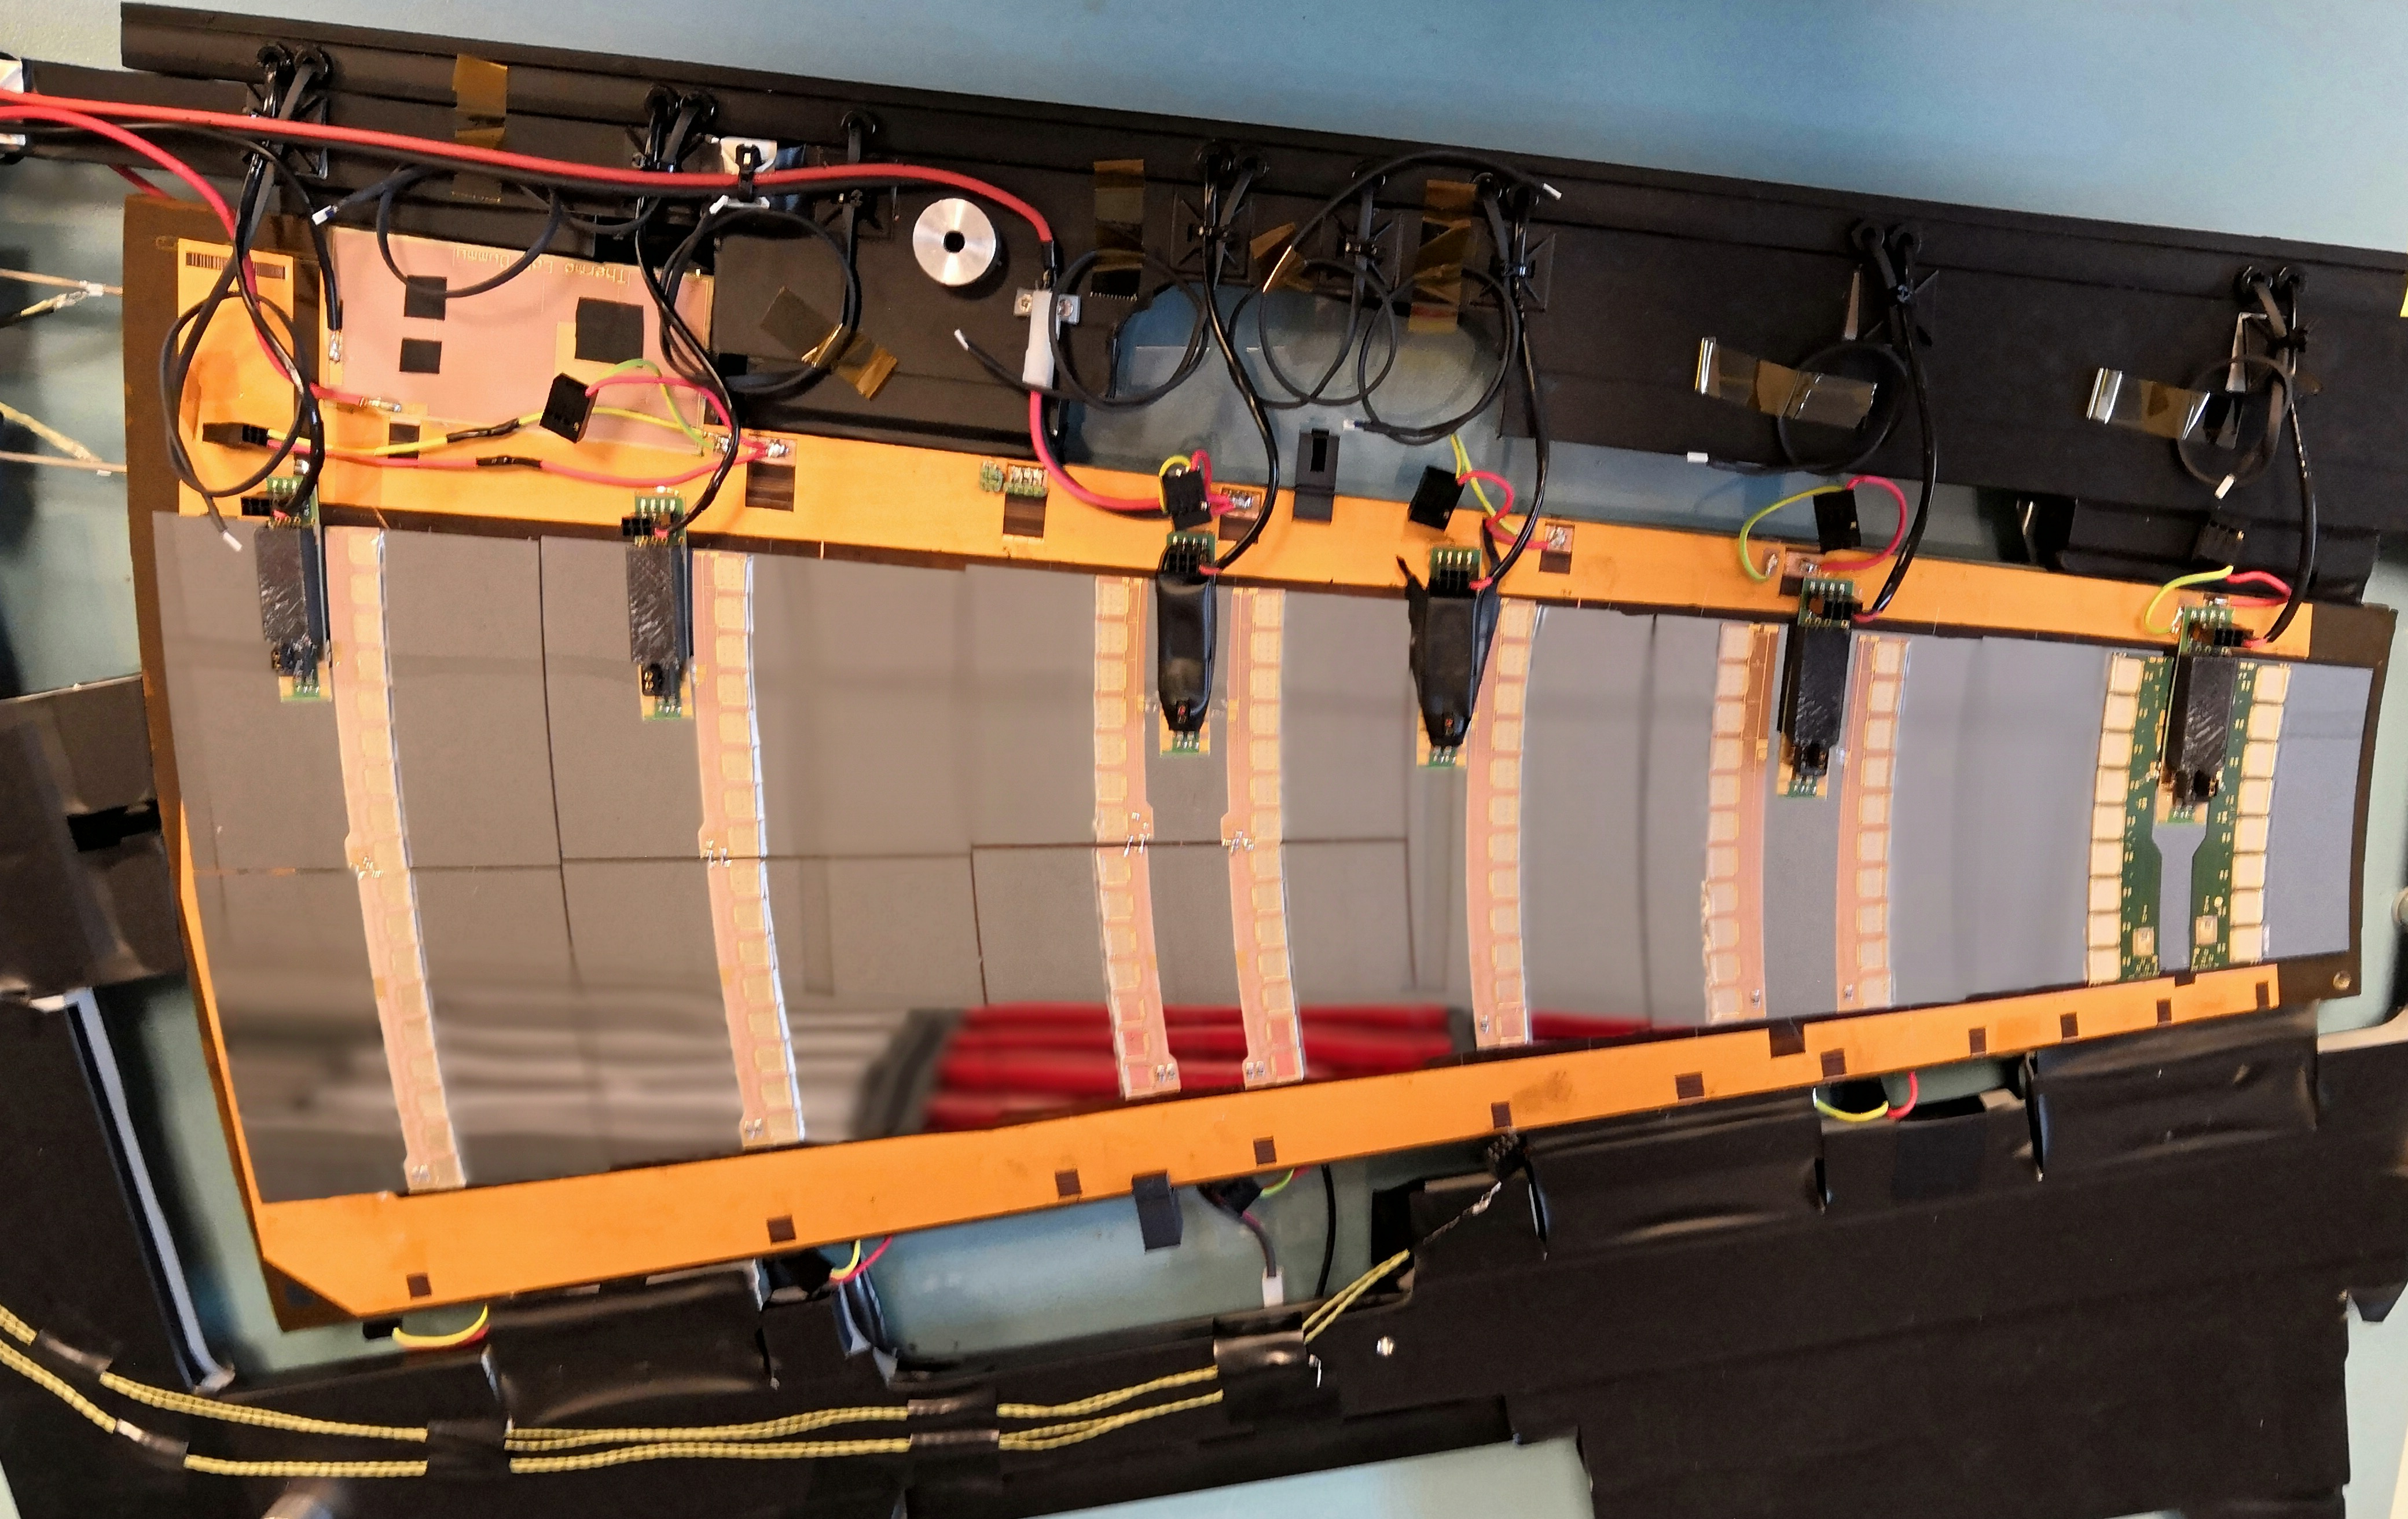
\includegraphics[width=\textwidth]{img/petal.jpg}
		\caption{Before}
		\label{}
	\end{subfigure} \hfill
	\begin{subfigure}{\textwidth}
		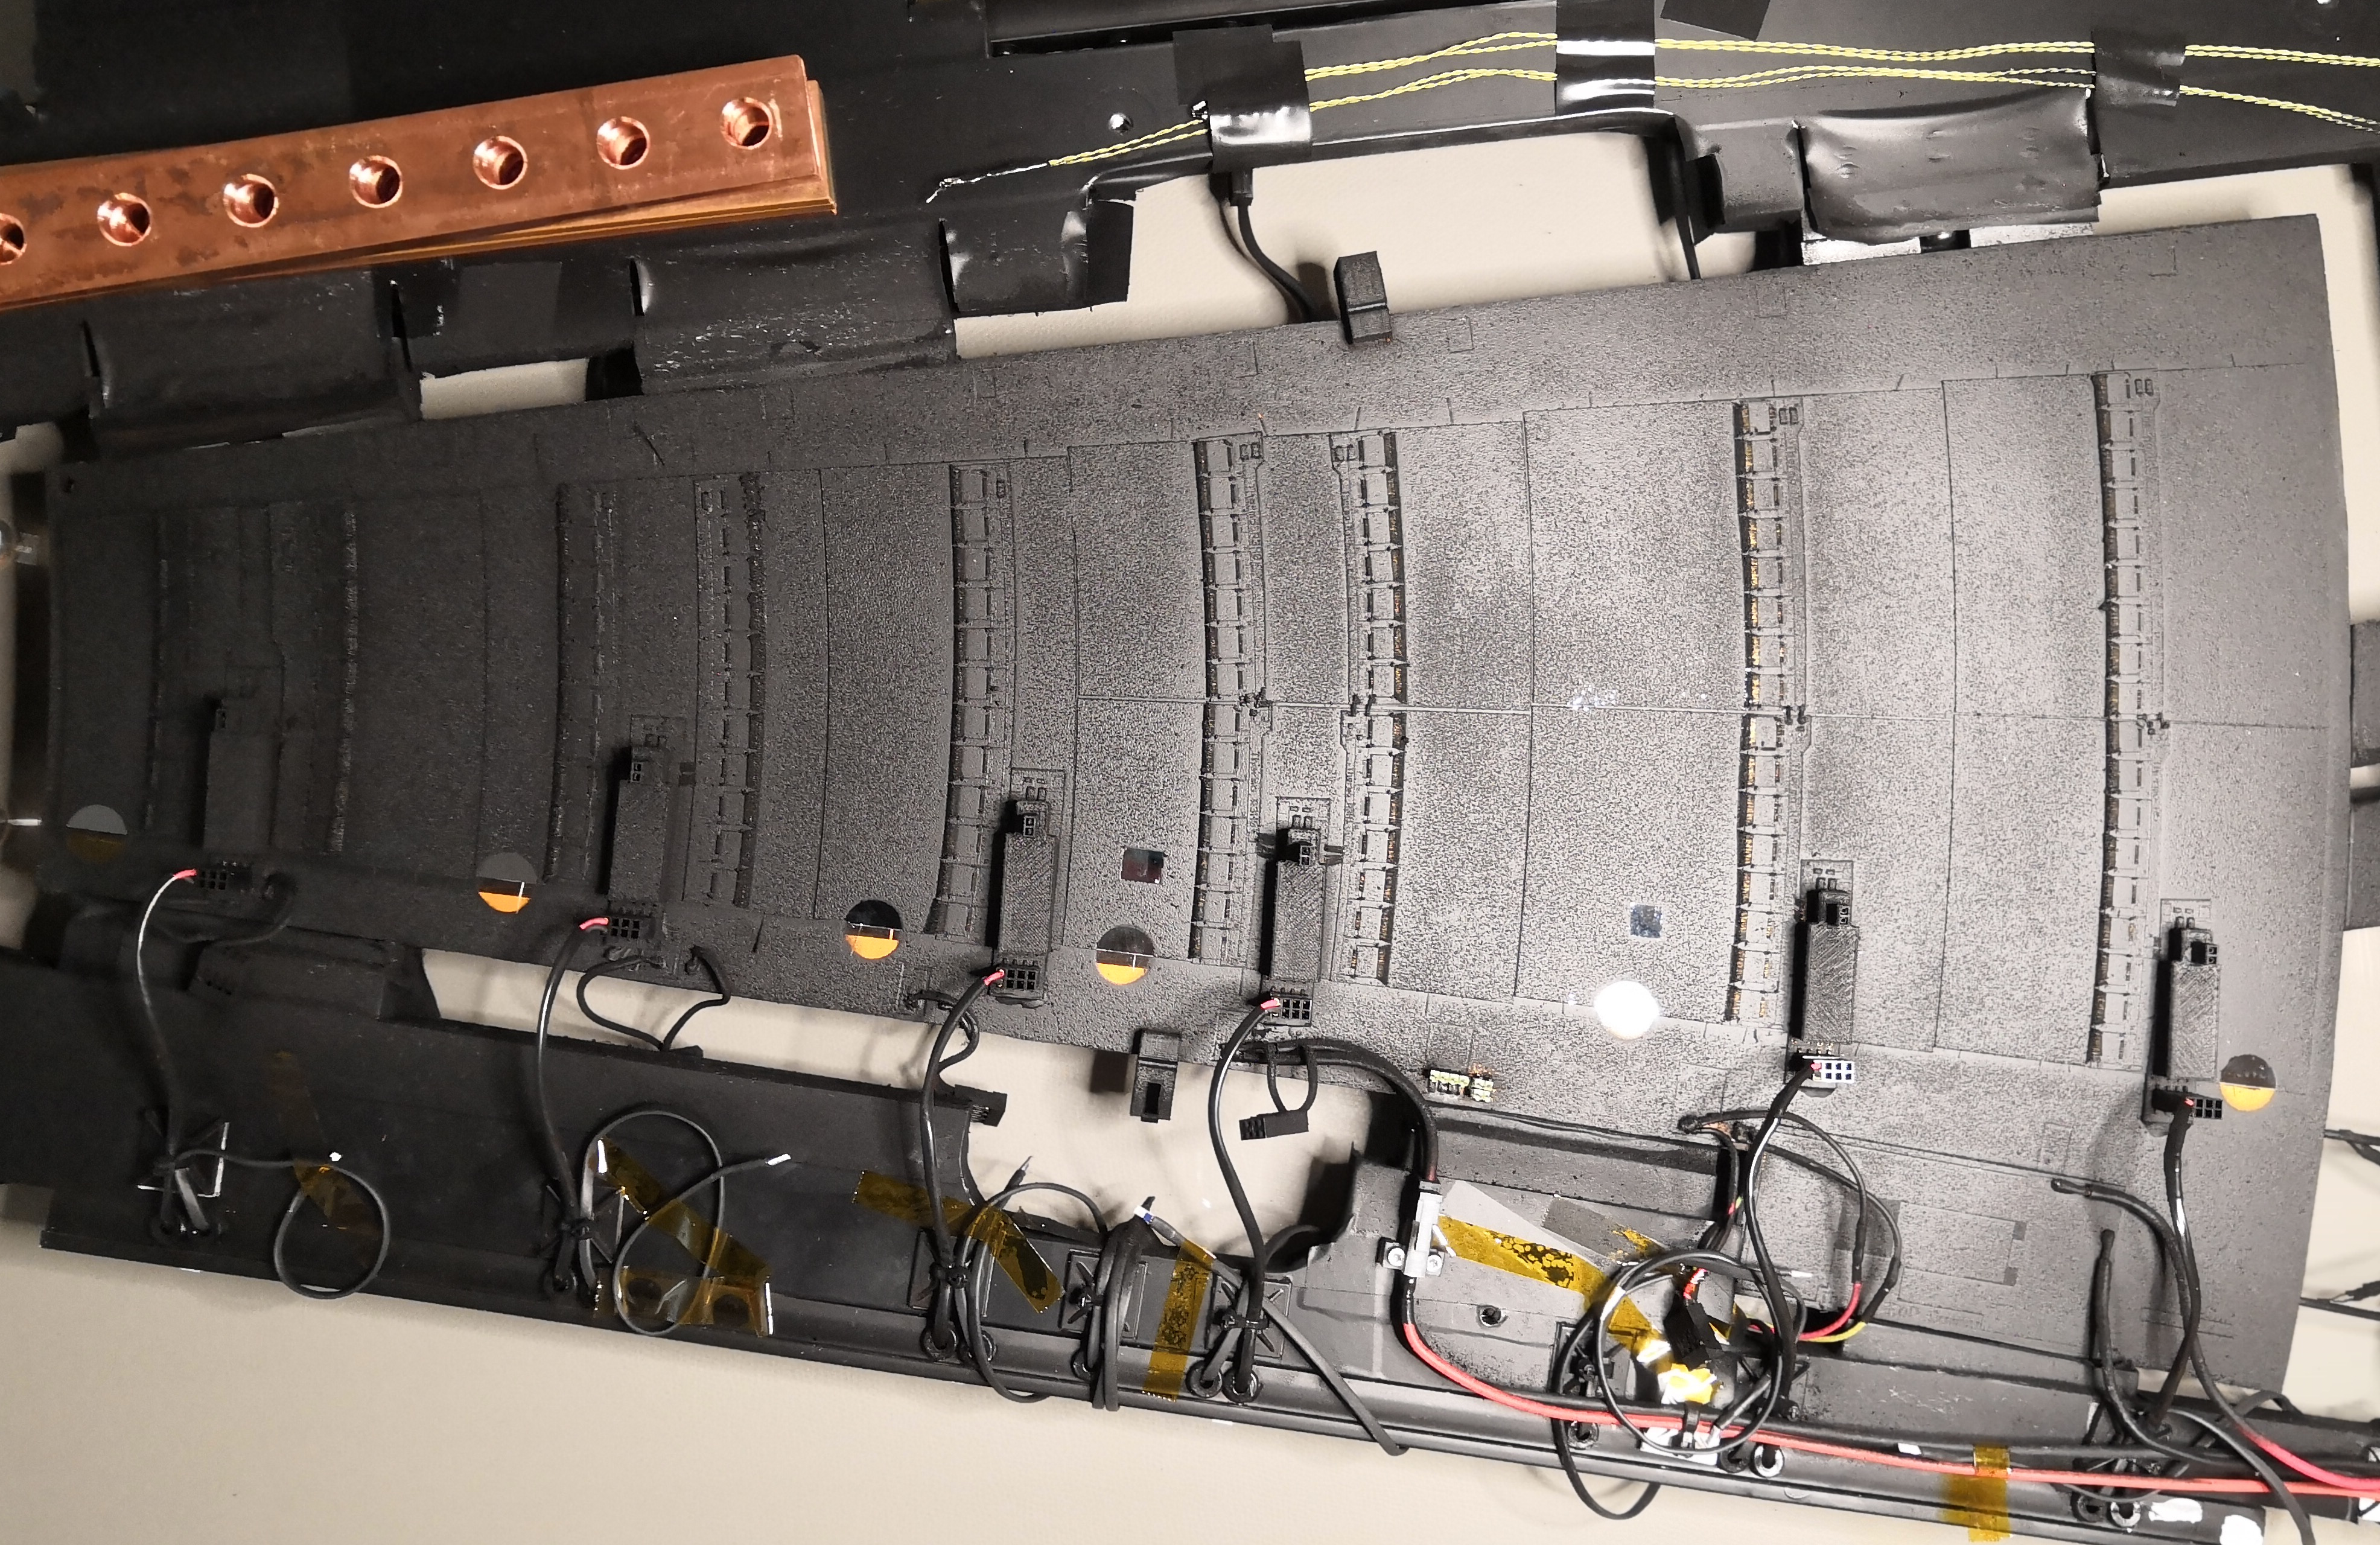
\includegraphics[angle=180, width=\textwidth]{img/entire.jpg}
		\caption{After}
		\label{}
	\end{subfigure}
	\caption{Petal before and after applying the paint.}
	\label{fig:petalPreAndPost}
\end{figure}
\begin{figure}[h!]
	\centering
	\includegraphics[angle=90, width=0.7\textwidth]{img/R3.jpg}
	\caption{Close up view of the paint structure.}
	\label{fig:petalCloseUp}
\end{figure}

\subsection{First Results}

\clearpage
\section{Summary and Outlook}
Following the rather detailed explanation in the foregoing sections, here is a summary of our results. \\


We did a variety of studies on the theoretical conversion between emitted IR radiation and object temperature. So far, the results are little satisfying. But, we are talking to Graham Beck and other teams involved in the inner tracker update and thermal performance tests. \\


We determined the emissivity of the paint in a range between 0.905 and 0.930. This result is coherent with our expectations but it needs to be narrowed some more to achieve a temperature uncertainty of less than \SI{1}{\degreeCelsius}. Given that the emissivity calculation is based on the conversion equation between radiant power and temperature further exploration in this direction needs to be done. \\


The camera software seems to overall give good results with some error, e.g. it overestimates the known emissivity of the tape by 0.01. \\


The petal was fully prepared for the measurements. After testing the trustworthiness of glueing the pt100s onto the Si, we successfully installed XX pt100s on the petal. Additionally, we sprayed the petal black. And even though the dried coating looks sandy, it fulfils its purpose. \\


Evtl.: First results. \\


In the future weeks, the ongoing measurements need to be analysed and evaluated. The final results are planned to be presented at the ??? in the beginning of October.

\end{document}
